

% This is sample.tex the demonstration file of
% MICCAI 2009 for Latex2e
% adapted from LLNCS.DEM from
% the LaTeX macro package from Springer-Verlag
% for Lecture Notes in Computer Science,
% version 2.2 for LaTeX2e
%
\documentclass{llncs}
%
\usepackage{algorithm}
\usepackage{algorithmic}
\usepackage{amssymb,amsmath}
\usepackage{makeidx}  % allows for indexgeneration
\usepackage{url}
\usepackage{dsfont}
\usepackage{wrapfig}
\usepackage{float}
\usepackage{subfig}
\usepackage{graphicx}

 \graphicspath{{pics/}{figures/}}

% list here all the paths to your figure folders

\renewcommand{\topfraction}{2}
\renewcommand{\dbltopfraction}{2}
\renewcommand{\bottomfraction}{2}
\renewcommand{\textfraction}{.0}
\renewcommand{\floatpagefraction}{2}
\renewcommand{\dblfloatpagefraction}{2}

\newcommand{\argmax}{\operatornamewithlimits{argmax}}
\newcommand{\argmin}{\operatornamewithlimits{argmin}}

\begin{document}
%
\frontmatter          % for the preliminaries
%
%\pagestyle{headings}  % switches on printing of running heads
\pagestyle{empty}  % switches on printing of running heads
%
\mainmatter              % start of your contributions
%
\title{Automated Quantification of Morphodynamics
for High-Throughput Live Cell Imaging Datasets}

%Automated Tracking and Segmentation of Phase-Contrast siRNA Sequences}
\titlerunning{Short Title} % abbreviated title (for running head)
%
%\author{author1\inst{1} \and author2\inst{1,2}  \and author3\inst{3}
\author{German Gonzalez\inst{1} \and Ludovico Fusco\inst{2} \and Olivier Pertz\inst{2} \and Kevin Smith\inst{1}}



\authorrunning{-}   % abbreviated author list (for running head)
%
%%%% modified list of authors for the TOC (add the affiliations)
% \tocauthor{author1 (Univesity of Author1),
% author2 (University of Author2),
% author3 (University of Author3),
% }
\tocauthor{-}

%\institute{Department of
%  Computer Science, University of Anonymous, UK, \email{author1@univ.edu},
%  \and
%  Department of Computer Science,  University of Anonymous2, USA.
%  \thanks{We are thankful to XYZ}
%}
 \institute{Computer Vision Lab, Ecole Polytechnique F\'ed\'erale de
   Lausanne, Switzerland
   \and
Institute of Biochemistry, University of Basel, Switzerland }
% anonymous stuff
%\author{-, -, -}
%\authorrunning{-}
%\tocauthor{-}
%\institute{-}
%\small{
% \institute{Computer Vision Lab., Ecole Polytechnique F\'ed\'erale de
  % Lausanne, Switzerland 
  % %\email{engin.turetken@epfl.ch}
  % \and
% ALBCOM, Universitat Polit\`ecnica de Catalunya, Barcelona, Spain
% }
%}
\newcommand{\comment}[1]{}
\maketitle              % typeset the title of the contribution

\begin{abstract}
%% -*- mode: latex; mode: reftex; mode: flyspell; TeX-master: "top.tex"; -*-

We  present  a  fully  automatic  method to  track  and  quantify  the
morphodynamics of  differentiating neurons in  fluorescence time-lapse
microscopy  datasets.    While  previous  efforts   have  successfully
quantified the dynamics of organelles  such as the cell body, nucleus,
or chromosomes of  cultured cells, neurons have proved  to be uniquely
challenging  due to  their  highly deformable  neurites which  expand,
branch, and collapse.  Our  approach is capable of robustly detecting,
tracking, and segmenting all the  components of each neuron present in
the sequence including the nucleus, soma, neurites, and filopodia.  To
meet  the   demands  required  for   high-throughput  processing,  our
framework is designed to be extremely efficient, capable of processing
a single image in approximately two seconds on a conventional notebook
computer.   For  validation  of  our approach,  we  analyzed  neuronal
differentiation datasets in  which a set of genes  was perturbed using
RNA interference. Our analysis confirms previous quantitative findings
measured  from   static  images,  as  well   as  previous  qualitative
observations of  morphodynamic phenotypes that could  not be measured
on a large scale. Finally,  we present new observations about the 
behavior of  neurons made  possible by our quantitative  analysis, which
are not immediately obvious to a human observer.

%  whose
%measurements were not feasible on a large scale.  Finally, using our
%quantitative analysis we make

%our dynamic
%quantitative analysis allows us to  make new observations that are not
%visible to a human observer.


%% we  use it to  perform an siRNA  screen and
%% successfully reproduce the findings of~\cite{}, which was performed at
%% steady-state under less stressful conditions [OLVIER, HELP US SAY THIS
%%   MORE  ELOQUENTLY].   Finally, we  apply  our  approach  to make  new
%% observations   based  on  dynamic   quantitative  analysis   that  was
%% previously impossible.

%% While  previous efforts
%% have tracked the soma and nucleus,  our approach is the first to fully automatically track
%% and reconstruct the neurites as  they expand, branch and collapse, and
%% to dynamically detect fine filopodia structures.

%We present a method to analyze and extract statistics from large-scale
%video sequences  of in-vitro neurons.   Our system is able  to detect,
%track, segment  and reconstruct each individual neuron  present on the
%videos.   We show how  such system  can be  used to  find correlations
%between neuron behaviour and the proteins used to mutate them.

%high throughput automation

%confirms pre-existing findings

%yields new understandings about the dynamic morphologies

%efficient, tracks, segments, and tracks neurites


\end{abstract}

\section{Introduction and Related Work}
\label{sec:intro}
%% -*- mode: latex; mode: reftex; mode: flyspell; TeX-master: "top.tex"; -*-


The  process  of forming  functional  connections  between neurons  is
complex  and   dynamic.   Time-lapse  microscopy   has  revealed  that
differentiating  neurons undergo  a large  range of  dynamic processes
including cell body motility, filopodial dynamics, and repeated cycles
of  neurite growth  and  retraction.  Of  critical  importance is  the
process  by which  axons and  dendrites are  formed in  which a neurite
ceases retracting, extends a   long  distance, and  forms
a connection. Such  dynamic events are  governed by a  complex protein
network that  coordinates   dynamic functions 
within the cytoskeleton, membrane, etc.

Powerful tools such as 
RNA interference  (RNAi)
technology,  fluorescent  protein   labeling,  image  processing,  and
automated high-throughput  microscopy have  opened the door  for large
scale  perturbation studies to help investigate such processes. RNAi  screens have  already led  to novel
insights   into  a  number   of  cellular   processes  such   as  cell
migration~\cite{Bakal07}  and endocytosis~\cite{Collinet10}.  However,
limitations  in  image  processing  have  restricted  most
investigations to static image analysis.

Knowledge  of dynamics is  essential if we are  to understand
complex  processes such  as neuron  morphogenesis.  However, designing
algorithms to quantify dynamic  behaviors is challenging, and
automatic methods  have appeared only  very recently. State-of-the-art
high-throughput techniques have successfully quantified morphodynamics
of  HeLA cancer  cells  in an  effort  to understand  the process  of
mitosis~\cite{Held10,Neumann10,Zhu05}.   However,  the morphology  and
dynamics of  these cell types  are relatively simple compared to neurons,
whose highly deformable  neurites  branch, expand,
retract, and collapse. 


In this paper, we  propose a  fully  automatic method  for  detecting, tracking,  and
segmenting {\em every component of the neuron} (nucleus,  soma, neurites, and filopodia), and quantifying  their dynamic behaviors in ways that were previously not possible. Our approach first  detects nuclei at each time step.  A greedy  tracking algorithm  associates detected nuclei belonging
belonging to the same neuron,  forming a list of detections corresponding  
to that neuron.  Using  the detected nuclei as seed  points, a region-growing
algorithm segments the neuron's soma.  The somata are used to
initialize a joint segmentation of the entire structure of all neurons
appearing in  a image using  a probabilistic method based  on shortest
path computations.   A  graph describing the  morphology of
the  neurites is extracted from  this segmentation.  Each neurite 
tree is tracked by association, and filopodia are detected
by analyzing the topology of the tracked neurites. Finally, 
a set of 156 {\em morphodynamic features} is extracted, quantifying
the behavior of the each neuron in the video.


As   demonstrated  in   Fig.~\ref{fig:video}, 
our  approach produces reliable  segmentations capable of capturing
complex  neuron  dynamics. To validate our approach, we analyzed a   
small-scale  siRNA screen  of 5  genes (3  siRNAs/gene). Our analysis
confirmed steady-state phenotypes obtained previously using 
MetaMorph\texttrademark~\cite{Pertz08}. We were also able to
quantify dynamic behaviors which had been previously observed, but never
measured~\cite{Pertz08}. Our  analysis also uncovered
new dynamic behaviors which are only apparant through dynamic analysis.

%While  our greedy tracking  and probabilistic  segmentation algorithms are  novel,  they are designed to be efficient and thus are relatively simple.  The  main contribution of this  paper is the  system as a whole,  which  is capable  of  high-throughput  processing of  videos, tracking individual  parts of  neurons, and quantifying  their dynamic behaviors in ways that were previously not possible.


%----------------------------------------------------------------------------
\begin{figure}[t]
       \begin{tabular}{@{\hspace{0mm}}c@{}|@{}c@{}}
        \includegraphics[width=45mm] {images/mv1_005.png}  &
        \includegraphics[width=45mm] {images/mv1_008.png} \\ [-.8ex]
        \hline \\ [-2.6ex]
        \includegraphics[width=45mm] {images/mv1_017.png}  &
        \includegraphics[width=45mm] {images/mv1_026.png} \\ [-.8ex]
        \hline \\ [-2.9ex]
       \end{tabular} 
       
      \begin{tabular}{@{\hspace{0mm}}c@{}c@{}c@{}c@{}}
        \includegraphics[width=22.5mm] {images/0_005.png} &
        \includegraphics[width=22.5mm] {images/0_008.png} & 
        \includegraphics[width=22.5mm] {images/0_017.png} & 
        \includegraphics[width=22.5mm] {images/0_026.png} \\ [-1ex]
        \includegraphics[width=22.5mm] {images/2_005.png} &
        \includegraphics[width=22.5mm] {images/2_008.png} & 
        \includegraphics[width=22.5mm] {images/2_017.png} & 
        \includegraphics[width=22.5mm] {images/2_026.png} \\ [-1ex]
        %\includegraphics[width=22.5mm] {images/3_005.png} &
        %\includegraphics[width=22.5mm] {images/3_008.png} & 
        %\includegraphics[width=22.5mm] {images/3_017.png} & 
        %\includegraphics[width=22.5mm] {images/3_026.png} \\ [-1ex]
        {\footnotesize $t = 50$ min} & 
        {\footnotesize $t = 80$ min} & 
        {\footnotesize $t = 170$ min} & 
        {\footnotesize $t = 260$ min} \\ [-1ex]
      \end{tabular}
    \vspace{-2mm}  
    \caption{ {\footnotesize {\it Neuron  Tracking Results.  } The top
        two rows  contain frames from an experiment  where MAP2K7 gene
        functions are inhibited.  For visibility we enhanced the image
        contrast.  Tracked neurons are marked by a unique color and id
        tag.   Nuclei  are denoted  by  filled  ellipsoids, somata  as
        contours,  and neurites  as trees.   Bottom rows  show details
        from  above: 1)  enhanced original  image 2)  tracked neurites
        marked with a different colors. Our  approach   performs  well  even  in  challenging
        situations where neurons appear in close proximity. Note: faintly  stained
        cells are ignored for robustness.}}
    \label{fig:video}
\vspace{-6mm}
\end{figure}
%----------------------------------------------------------------------------




%\section{Related Work}
%\label{sec:related}
%%% -*- mode: latex; mode: reftex; mode: flyspell; TeX-master: "top.tex"; -*-


\vspace{-3mm}
\section{High-throughput Tracking and Segmentation}
\label{sec:method}
%% -*- mode: latex; mode: reftex; mode: flyspell; TeX-master: "top.tex"; -*-

\vspace{-3mm}

The input to our approach is a series of $T$
images $\mathcal{I} = \{I_1, \ldots, I_t, \ldots,
I_T\}$ from which we extract $K$ nucleus
detections $d_t^k$.  The tracking step described
in Sec.~\ref{sec:tracking} associates valid
detections across time steps while rejecting
spurious detections. Since each neuron contains
only one nucleus, there is a one-to-one mapping
between each valid nucleus detection $c_t^i$ and a
neuron $X_t^i$.  Thus, the tracking task is to
provide a set of neuron detections $\mathcal{X}^i
= \{X_{a}^i,\ldots,X_t^i,\ldots,X_{b}^i \}$
defining an individual neuron $i$ from time $t=a$
to $t=b$.  As depicted in Fig.~\ref{fig:notation},
each neuron detection $X_t^i$ is composed of a
nucleus $c_t^i$, a soma $s_t^i$, a set of $J$
neurites $\{n_t^{i,1}, \ldots, n_t^{i,j}, \ldots,
n_t^{i,J} \}$, and a set of $L$ filopodia
associated with each neurite $F_t^{i,j} =
\{f_t^{i,j,1},\ldots,f_t^{i,j,l},\ldots,f_t^{i,j,L}
\}$ so that $N_t^i = \{( n_t^{i,1},F_t^{i,1}),
\ldots,(n_t^{i,j},F_t^{i,j}) \}$.  Thus, a
complete neuron $i$ at time step $t$ is described
by $X_t^i = \{ c_t^i, s_t^i, N_t^i \}$.


\vspace{-3mm}
\subsection{Nuclei and Somata Detection and Segmentation}
\vspace{-2mm}
\label{sec:detection}
%% \vspace{-2mm}
The first step in our approach is to extract a set
of nucleus detections $\{d^1,\ldots,d^K\}$ over
the image series. We worked with two-channel
images where the cytoskeleton is marked with
Lifeact-GFP and nuclei are marked with
NLS-mCherry. The nuclei can be reliably detected
and segmented by simply thresholding the
NLS-mCherry channel and performing a morphological
filling operation.  Alternatively, one could apply
a fast machine learning detector such as the one
in~\cite{Smith09}.


Using the nuclei as seed points, somata are
segmented as follows.  A list of pixels
neighboring the current soma segmentation is
maintained.  At each iteration, the neighbor with
the smallest weighted distance to the centroid of
the seed nucleus detection $D = \lambda || u -
d^k|| + |I(u) - \hat{I}(d^k)|$ is added to the
soma so long as $D < Y$, where $u$ is a location
in the image, $I(u)$ is the pixel intensity at
that location, $\hat{I}(d^k)$ is the mean
intensity of detection $d^k$, and $Y$ is a
threshold.


\vspace{-3mm}
\subsection{Efficient Tracking of Nucleus Detections}
\label{sec:tracking}
\vspace{-2mm}

The tracking algorithm searches through the full
set of nuclei detections and iteratively
associates the most similar pairs of detections,
returning lists of valid detections corresponding
to each neuron $\mathcal{X}^i$.  This is
accomplished by constructing a graph
$\mathcal{G}=(\mathcal{D},\mathcal{E})$ where each
node $d^k_t \in \mathcal{D}$ corresponds to a
detection.  For each detection $d^k_t$ in time
step $t$, edges $e \in \mathcal{E}$ are formed
between $d^k_t$ and all past and future detections
within a time window $W$.  A weight $w_e$ is
assigned to each edge $e^{k,l}$ connecting $d^k_t$
and $d^l_t$. The weight $w_e$ relates to spatial
distances, temporal distances, and a shape
measure: $w_{e} = \alpha || d^k_{t1} - d^l_{t2} ||
+ \beta |t1 - t2| + \gamma f(\nu^k_{t1},
\nu^l_{t2})$, where $\nu^k$ is a shape feature
vector containing $d^k_t$'s area, perimeter, mean
intensity, and major and minor axis lengths of a
fitted ellipse. $f$ evaluates differences between
a feature $a$ extracted from $d^k_t$ and $d^l_t$
as $f(a^k,a^l) = {|a^k - a^l|}/{|a^k + a^l|}$.
The tracking solution corresponds to a set of
edges $\mathcal{E'} \subset \mathcal{E}$ with
maximal edge weight $Q$ that forms a set of
disconnected tracks $\mathcal{T}$ and minimizes
the cost function $\sum_{e \in \mathcal{T}} w_e$.

To minimize this cost function, we adopt a greedy
selection algorithm, summarized in
Fig.~\ref{fig:greedytracking}, that iteratively
selects an edge with minimum cost $\hat w_e$ and
adds it to the set $\mathcal{L}$ removing future
and past connections from the detections $e^{k,l}$
connects.  The algorithm iterates until the
minimum cost $\hat w_e$ is greater than a
threshold $Q$.  Each track $i$ is then associated
with a neuron identity $\mathcal{X}^i$.




%----------------------------------------------------------------------------
\begin{figure}[t]
  \begin{center}
       \begin{tabular}{@{\hspace{-1mm}}c}
        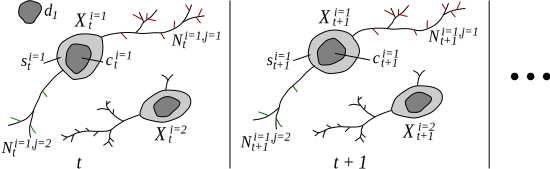
\includegraphics[width = 87mm] {images/neurondrawing.pdf}\\ [-2.4ex]
       \end{tabular} 
    \caption{ \footnotesize Neuron tracking
      notation.  At time $t$ a neuron $i$
      detection $X_t^i = \{ c_t^i, s_t^i, N_t^i
      \}$ contains a nucleus $c_t^i$, a soma
      $s_t^i$, and a set of neurite-filopodia
      tuples $N_t^i = \{( n_t^{i,1},F_t^{i,1}),
      \ldots,(n_t^{i,j},F_t^{i,j}), \ldots,
      (n_t^{i,J},F_t^{i,J}) \}$ which contains $J$
      neurites and their associated filopodia
      shown in red for $j=1$ and green for
      $j=2$. A spurious nucleus detection $d_1$ is
      also shown.  A neuron $i$ is defined by a
      time-series of neuron detections
      $\mathcal{X}^i =
      \{X_{a}^i,\ldots,X_t^i,\ldots,X_{b}^i \}$.
      The tracking returns a set $\mathcal{X}^i$
      for each neuron. }
    \label{fig:notation}
  \end{center}
\vspace{-8mm}
\end{figure}
%% by linking nucleus detections  and ``growing'' the
%%         neuron from the nucleus seed
%----------------------------------------------------------------------------







\vspace{-3mm}
\subsection{Neuron Segmentation and Neurite Tree Extraction}
\label{sec:segmentation}
\vspace{-2mm} Given an image $I_t$ and the set of
somata present in it $S_t=\{s_t^1 \dots s_t^m \}$,
our goal is to associate to each pixel $u$ a label
$J_t(u)$ that indicates to which neuron (soma) it
belongs, if any.  The probability of $J_t(u)$ can
be deduced using Bayes' rule,
\begin{equation}
  \label{eq:bayes}
  P(J_t(u)=i|S_t,I_t) = \frac{P(S_t,I_t| J_t(u)=i)}{\sum_{\eta=1}^m P(S_t,I_t|J_t(u)=\eta)},
\end{equation}
\noindent where we assume a uniform distribution
on $P(J_t(u))$.  The numerator is modeled as the
probability of the path $L$ that connects
maximally pixel $u$ to soma $s_t^i$, $ P(S_t,I_t|
J_t(u)=i) = \max_{L:u\rightarrow s_t^i}
\prod_{\{l_{r}\} \in L } P(I_t(r)|l_{r}),$ where
$l_{r}$ are indicator variables for the locations
forming the path $L$.  We chose this model since
it produces connected components and an optimal
maxima can be found by minimizing its negative
likelihood using Dijkstra's shortest path.

To optimize this function, we map the image $I_t$
to a graph $\mathcal{G}_t^i = (V,E)$ whose
vertices $u$ are the pixels in $I_t$ and whose
directed edges $e_{r,v}$ connect each pixel to its
four neighbors.  We assign to each edge a weight
$w_{r,v} = -log P(I_t(v)|v)$.  $P(I_t(v)|v)$
represents the probability that a neurite
traverses a node $v$.  It is obtained by applying
a sigmoid function to the output of the tubularity
filter of~\cite{Frangi98}.  The parameters of the
sigmoid function are estimated using maximum
likelihood. Finally, we define the set of neurite
pixels $U_n^t$ as those that connect to any soma
with a higher probability than $\epsilon$.  We
predict their labels as the ones that maximize
Eq.~\ref{eq:bayes}.  The set of pixels associated
to neuron $X_t^i$ is the union of the neurites and
the soma associated with $i$, $ U_i^t = \{u \in
U_n^t | J_t(u) = i\} \cup s_t^i$. To reduce the
neurite segmentation to a tree, we skeletonize the
neuron and define as root node the pixel of the
skeleton closest to the centroid of the nucleus.
We instantiate a Minimum Spanning Tree from the
root and create a neurite tree whenever the
spanning tree exits the soma.




\subsection{Neurite Tracking and Filopodia Detection}
\label{sec:neurite}
\vspace{-2mm} The identity of neurites is tracked
across the frames of the time-lapse videos by
applying the algorithm described in
Sec~\ref{sec:tracking}, but using the centroids of
the neurite trees instead of the centroids of
nuclei, with the additional constraint that edges
may only exist between neurites that emanate from
the same soma.  Filopodia are detected by starting
at each leaf node in a neurite and traversing the
tree until a branch point is reached. If the
distance traversed is less than a threshold $T_f$,
the traversed locations are considered to be
filopodia.


%----------------------------------------------------------------------------
\begin{figure}[t]
  \centering
       \begin{tabular}{@{\hspace{-1mm}}c@{}}
        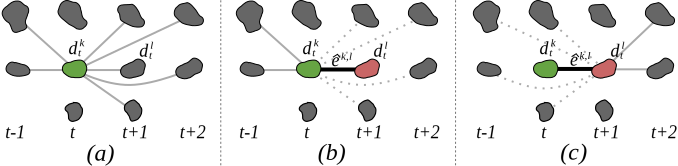
\includegraphics[width = 85mm] {images/greedytracking.pdf}\\ [-2.4ex]
       \end{tabular} 
    \caption{ \footnotesize Efficient tracking by
      association.  {\em (a)} A graph is built by
      fully connecting each detection to all
      future and past detections within a time
      window $W$.  In this simplified diagram,
      only $d^k_t$'s edges are shown and
      $W$=2. {\em (b)} Each iteration, the edge
      $\hat{e}^{k,l}$ with minimum cost
      $\hat{w}_e$ is added to $\mathcal{E}'$.
      Edges connecting $d^k_t$ to future
      detections are removed from $\mathcal{E}$.
      {\em (c)} Edges connecting $d^l_t$ to the
      past are removed from $\mathcal{E}$.  The
      process is repeated until $\hat w_e > Q$. }
    \label{fig:greedytracking}
%\vspace{-4mm}
\end{figure}
%----------------------------------------------------------------------------


%%----------------------------------------------------------------------------
%\begin{figure}[t]
%  \centering
%       \begin{tabular}{@{\hspace{-1mm}}c@{}}
%        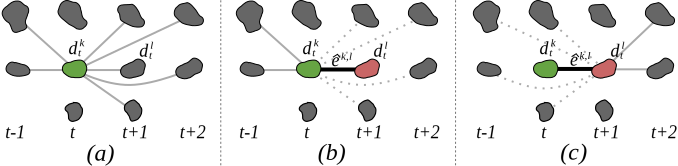
\includegraphics[width = 85mm] {images/greedytracking.pdf}\\ [-2.4ex]
%       \end{tabular} 
%    \caption{ \footnotesize Efficient tracking by association.  {\em  (a)} A graph is
%	built where each detection is fully connected to all future and past detections 
%within  a time  window  $W$.  In this diagram, only  $d^k_t$'s edges  are
%        shown and $W$=2. {\em  (b)} Each iteration,  the edge $\hat{e}^{k,l}$
%        with   minimum  cost   $\hat{w}_e$  is  added  to $\mathcal{E}'$.   Edges  connecting
%        $d^k_t$ to  future detections are  removed from $\mathcal{E}$.
%        {\em  (c)} Edges  connecting  $d^l_t$ to  the past  are
%        removed from $\mathcal{E}$.  The process is repeated until $\hat w_e > Q$. }
%    \label{fig:greedytracking}
%\vspace{-4mm}
%\end{figure}
%%----------------------------------------------------------------------------

%%-----------------------------------------------------------------
%\begin{algorithm}[b]
%\caption{Tracking association algorithm}
%\footnotesize
%\begin{algorithmic}[100]
%\STATE Start with an empty set $\mathcal{E}'$.
%\REPEAT
%\STATE Find edge $\hat e^{k,l}$ with minimum cost $\hat w_e$.
%\STATE Add $\hat e^{k,l}$ to $\mathcal{E}'$, linking detections $d^k_{t1}$ and $d^l_{t2}$.
%\STATE Remove $\hat e^{k,l}$ from $\mathcal{E}$.
%\IF {$ t1 < t2 $}
%\STATE Remove edges between $d^k_{t1}$ and {\em future} detections (where $t > t1$) from $\mathcal{E}$
%\STATE Remove edges between $d^l_{t2}$ and {\em past} detections (where $t < t2$) from $\mathcal{E}$
%\ELSE
%\STATE Remove edges between $d^k_{t1}$ and {\em past} detections (where $t < t1$) from $\mathcal{E}$
%\STATE Remove edges between $d^l_{t2}$ and {\em future} detections (where $t > t2$) from $\mathcal{E}$
%\ENDIF
%\UNTIL{$\hat w_e > Q$}
%\end{algorithmic}
%\normalsize
%\label{algo:greedy}
%\end{algorithm}
%%-----------------------------------------------------------------


\vspace{-3mm}
\section{Extracting Morphodynamic Features}
\label{sec:features}
%% -*- mode: latex; mode: reftex; mode: flyspell; TeX-master: "top.tex"; -*-
\vspace{-3mm} Our  tracking and  segmentation method produces  sets of
graphs linking  detections, contours, and trees to  define each neuron
over  time.  This  data   structure  is  not  immediately  useful  for
quantifying dynamic behaviors.  To facilitate the analysis, we extract
a  set of {\em  156 meaningful  features} from  our data  structure to
quantify morphodynamics, which  are too numerous to list  here.  A few
examples  for   the  nucleus   and  soma  include:   area,  perimeter,
Lifeact-GFP  intensity,  NLS-mCherry  intensity, speed,  acceleration,
total distance  traveled, time spent  expanding/contracting, frequency
of expansion.  For neurites: number  of branches, distance from tip to
soma, filopodia  length, number of  filopodia, major axis,  minor axis
and eccentricity of an ellipse fitted to the neurite, total length, time
spent expanding/contracting, frequency of expansion (and
$\Delta$'s for all above).



\vspace{-3mm}
\section{Results and Conclusion}
\label{sec:results}
%% -*- mode: latex; mode: reftex; mode: flyspell; TeX-master: "top.tex"; -*-
\vspace{-3mm}
%----------------------------------------------------------------------------
\begin{figure}[t!]
  \centering
       \begin{tabular}{@{\hspace{-2mm}}c@{\hspace{2mm}}c@{}}
         {\tiny (a) Maximum Distance from Neurite Tip to Soma} &
         {\tiny (b) $\Delta$ Eccentricity of an Ellipse Fitted to Neurite} \\
        \includegraphics[height = 41mm] {images/DistToSomaExtremeNeurite.pdf} &
        \includegraphics[height = 41mm] {images/EccentricityNeuriteDelta.pdf} \\ [-1ex]
        {\tiny $\mu m$} & \\
        {\tiny (c) Nucleus Speed} &
        {\tiny (d) Maximum Number of Branches in Neurite} \\ [-1ex]
        \includegraphics[height = 41mm] {images/SpeedNuclei.pdf} &
        \includegraphics[height = 41mm] {images/MaxBranchCountNeurite.pdf} \\ [-1ex]
        {\tiny $\mu m$/min } & \\ [-2.2ex]
       \end{tabular} 
    \caption{    {\footnotesize   {\it    Quantitative   Morphodynamic
          Analysis.}  Four   informative  morphodynamic  features  are
        plotted, where the control  experiment is marked in gray below
        the  siRNA  targets.   Black  dots  represent  collected  data
        points.  Red  bars  indicate  the mean,  green  bars  indicate
        standard deviation.  The blue line shows the  control's mean for
        comparison. Values under the $\%$ column are the percentage of
        data  points  above  the  control's  mean.  Values  under  $P$
        indicate the student-t test $p$-value. See text for details.}}
    \label{fig:quantitative_analysis}
    \vspace{-7mm}
\end{figure}
%% by linking nucleus detections  and ``growing'' the
%%         neuron from the nucleus seed
%----------------------------------------------------------------------------



\noindent  {\bf Experimental  Setup and  Methodology --}  We  used our
method to perform a small-scale siRNA screen in which the functions of
5  genes were inhibited  with three  goals in  mind: to  reproduce the
findings of~\cite{Pertz08}, to confirm previous qualitatively observed
morphodynamics, and  to uncover  new dynamic behaviors.   Three siRNAs
were applied for each gene  (SrGAP2, MAP2K7, RhoA, Trio, and Net), for
a  total  of 17  experiments  including  2  controls.  30  videos  per
experiment were obtained over the  course of 3 days, with images taken
in  10 minute intervals  for a  total of  510 videos,  each containing
approximately 100 2-channel images  of $696 \times 520$ resolution.  A
total of 7,298 neurons and 33,213 neurites were tracked and segmented.
Our method  processes a single video  in 210 seconds on  a Lenovo W510
notebook computer (2.1  seconds per image), and the  entire screen was
processed in parallel in just a few hours using conventional PCs.

%over the course  of 16 to 18 hours,

Our  quantitative  analysis  investigated  the effects  of  inhibiting
various gene  functions on each  of the 156 morphodynamic  features we
extracted     from    our     segmentations     as    described     in
Sec.~\ref{sec:features}.   We  summarize  our  findings below  and  in
Fig~\ref{fig:quantitative_analysis}. We also  provide a detailed table
and  video  results in  the  supplementary  material.  Throughout  the
pipeline, many potential sources of noise exist, including variability
in   neuron   behavior,   transfection   effects,  mistakes   in   our
segmentation, and  imaging conditions.  The sheer number  of cells and
neurites  analyzed  helps  to  average  out the  noise.  Our  findings
reported  below are statistically  significant, all  having $p$-values
$<< 0.05$.

\vspace{3mm}
\noindent {\bf Analysis --} Our analysis confirms the effects found through static image
analysis  in~\cite{Pertz08}.  In  particular,  RhoA  loss  of  function
resulted in fewer but longer neurites than the control. SrGap loss was
found to have longer neurites, and  Map2K7 loss was found to have
more neurites but with short length.  These findings  were confirmed by dynamic measures in
our experiments: the mean longest  neurite length -- control $22.6 \mu
m$, RhoA-3 $32  \mu m$, SrGap2-1 $28.9 \mu m$,  and Map2K7-1 $19.5 \mu
m$  (see  Fig.~\ref{fig:quantitative_analysis}a)$^1$;  and  by  a  dynamic
measure --  the mean  number of neurites  belonging a neuron  over its
lifetime: control 3.4, RhoA 3.1, and Map2K7-1 3.9.

It  was qualitatively  observed, but  never quantified,  that  loss of
SrGap2 function  produces a  high number of  filopodia, and  that RhoA
loss  results  in neurites  that  easily  extend  but have  difficulty
retracting. These morphodynamics were  confirmed by our analysis. Mean
number of filopodia detected per  neurite over its lifetime was $6.69$
in the control  and $8.81$ for SrGap-3$^1$. The  mean change in elongation
as measured  by an ellipse fitted  to the neurite was  $5.7\%$ for the
control        and        $5.3\%$        for        RhoA-1        (see
Fig.~\ref{fig:quantitative_analysis}b)$^1$. While this difference may seem
small,  it is  significant due  to the  large amount  of  data collected
($p$-value is $2 \times 10^{-7}$).

Our quantitative analysis revealed new morphodynamics which
were not obvious to human  observers. We found that RhoA function loss
slowed  neuron motility and  Map2K7 increased  it.  Control cells
moved at  .30 $\mu  m / min$,  RhoA moved  at .23 $\mu  m /  min$, and
Map2K7-2     moved     at    .37     $\mu     m     /    min$     (see
Fig.~\ref{fig:quantitative_analysis}c).  We  also found that  RhoA and
SrGap  increased the  branching of  the
neurites (see Fig.~\ref{fig:quantitative_analysis}d).  Over the course
of a  neurites lifetime, the maximum  number of branches  in a control
neuron    was    14.5,   19.44    for    RhoA-3,    and   21.39    for
SrGap2-3\footnote{Only neurons containing  the  $10^{th}$  percentile  of
  longest neurites were considered.}.

\vspace{3mm}
\noindent {\bf Conclusion  --} We have described a  set of algorithms
which, as a  system, are capable of robustly  tracking and segmenting entire
neurons  including  the nucleus,  soma,  neurites  and filopodia.  Our
approach is efficient, and  can analyze high-throughput datasets using
meaningful dynamic  features extracted from  our segmentations.
We  validated  our  approach  by  reproducing
previous findings,  confirming anecdotal findings,  and uncovering new
dynamic phenotypes. It is beyond the scope of this work to comment on
the biological significance of these findings, if there is any. We
leave that for future work.


%% Our approach
%% is designed to be efficient for analyzing high-throughput 
%% datasets.
%% a series of algorithm that
%% we presented

%% whole system
%% efficient

%% system is validated thorugh corroboration previous findings
%% confirmed anectocla findings
%% uncovered new dynamic phenotypes

%% biological context out of scope, future work will concentrate on that
%and addressing failure modes

%Our could be applied many other screens do more serious investiagation.


%% max branching points over  neurite lifetime
%% control  14.55
%% RhoA-3  19.44
%% SrGap2-3  21.39

%% speed
%% control   $ 9.91  \mu m / s $
%% RhoA-2    7.45
%% SrGap2-2    11.78
%% Map2K7-2   0.37
%%  0.3097    0.2328    0.3681


% eccentricity per neurite per time frame
% control 0.82
% RhoA-2 0.843  p-value  $4 \times 10^{-74}$

%% delta eccentricity
%% RhoA-1 $5.3\%$ change  $p-value$ $2 \times 10^{-7}$
%% Control $5.7\%$ change


%% over lifetime
%% RhoA_1 3.1 
%% Control 3.4
%% SrGap2_1 4.1  
%% Map2K7_1 3.9

%% 6.7 filo/neurite control



%supplementary material

%% say  how high throughput  gets rid  of noise,  and makes  our findings
%% statistically significant. talk about many sources of noise


%% p-value





%% note: make sure to say that we do not track everything - only reliably stained cells.

%% how long does it take to process?
%% It takes approximately 2.26 seconds to process each frame on a Lenovo W510 notebook computer.

%% image 97 frames 10 minute interval, 16 to 18 hours

%% In  total,  we   analyzed  $420$  video  sequences.







%\subsection{Experimental Methodology}

%\subsection{Biological Conclusions}


%\section{Conclusion}
%\label{sec:discussion}
%\input{discussion.tex}

\vspace{-4mm}
\bibliographystyle{splncs}
\footnotesize{
\bibliography{short,vision,misc,biomed}
% \bibliography{sample}
}
\end{document}








